%!LW recipe=pdflatex

\documentclass{standalone}

\usepackage{animate}
\usepackage{amsmath, amssymb, amsthm, mathrsfs, amsfonts, dsfont}
\usepackage{ascmac}
\usepackage{bbm}
\usepackage{bm}
\usepackage{breakcites}
\usepackage{calc}
\usepackage[style=base]{caption}
\usepackage{enumerate}
\usepackage[T1]{fontenc}
\usepackage{ifthen}
\usepackage{mathtools}
\usepackage{makecell}
\usepackage{mlmodern}
\usepackage{newtxtext}
\usepackage{optidef}
\usepackage{physics}
\usepackage{pifont}
\usepackage{setspace}
\usepackage{stfloats}
\usepackage{subcaption}
\usepackage{svg}
\usepackage{tikz}
\usepackage{xparse}
\usepackage[all]{xy}

\usepackage{float}
\usepackage{color}
\usepackage{graphicx}
\usepackage[colorlinks=true, allcolors=blue]{hyperref}


% === Commands ===

\definecolor{cA}{HTML}{0072BD}
\definecolor{cB}{HTML}{EDB120}
\definecolor{cC}{HTML}{77AC30}
\definecolor{cD}{HTML}{D95319}
\definecolor{cE}{HTML}{7E2F8E}
\newcommand{\cAText}[1]{\textcolor{cA}{#1}}
\newcommand{\cBText}[1]{\textcolor{cB}{#1}}
\newcommand{\cCText}[1]{\textcolor{cC}{#1}}
\newcommand{\cDText}[1]{\textcolor{cD}{#1}}
\newcommand{\cEText}[1]{\textcolor{cE}{#1}}
\newcommand{\red}[1]{\textcolor{red}{#1}}
\newcommand{\blue}[1]{\textcolor{blue}{#1}}
\newcommand{\green}[1]{\textcolor{green}{#1}}
\newcommand{\gray}[1]{\textcolor{gray}{#1}}
\newcommand{\black}[1]{\textcolor{black}{#1}}

\usetikzlibrary{
  3d,
  fit,
  calc,
  math,
  matrix,
  patterns,
  backgrounds,
  arrows.meta,
  decorations.pathmorphing,
}

\begin{document}
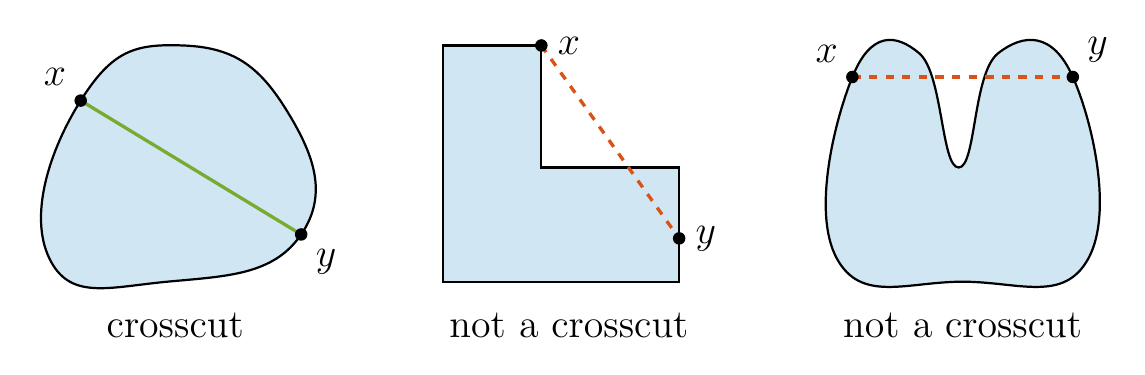
\begin{tikzpicture}[
    scale=1,
    K/.style={thick, draw=black, fill=cA!18},
    crosscut/.style={very thick, draw=cC},
    noncrosscut/.style={very thick, draw=cD, dashed},
    pt/.style={circle, fill=black, inner sep=1.6pt},
    lab/.style={font=\Large},
    note/.style={font=\Large, align=center}
]

% ============================================================
% Example 1: crosscut
% x,y are exactly vertices on bd K.
% The open segment intv xy lies inside int K.
% ============================================================
\begin{scope}[shift={(0,0)}]
    \coordinate (A1) at (0.0,0.3);
    \coordinate (B1) at (0.4,2.3);
    \coordinate (C1) at (1.7,3.0);
    \coordinate (D1) at (3.0,2.2);
    \coordinate (E1) at (3.2,0.6);
    \coordinate (F1) at (1.5,0.0);

    \draw[K]
        plot[smooth cycle, tension=0.85] coordinates {
            (A1) (B1) (C1) (D1) (E1) (F1)
        };

    % x,y are chosen as named boundary points
    \coordinate (x1) at (B1);
    \coordinate (y1) at (E1);

    \draw[crosscut] (x1) -- (y1);

    \node[pt,label={[lab]above left:$x$}] at (x1) {};
    \node[pt,label={[lab]below right:$y$}] at (y1) {};

    \node[lab] at (1.6,-0.55) {crosscut};
\end{scope}

% ============================================================
% Example 2: not a crosscut
% x is exactly a corner of bd K, y is exactly on bd K.
% The segment enters K through the corner x and crosses bd K only once more
% before reaching y; hence part of intv xy is outside K.
% ============================================================
\begin{scope}[shift={(5.0,0)}]
    % A polygonal K with an inward corner at x
    \coordinate (A2) at (0.0,0.0);
    \coordinate (B2) at (0.0,3.0);
    \coordinate (x2) at (1.25,3.0);
    \coordinate (C2) at (1.25,1.45);
    \coordinate (D2) at (3.0,1.45);
    \coordinate (E2) at (3.0,0.0);

    \draw[K] (A2) -- (B2) -- (x2) -- (C2) -- (D2) -- (E2) -- cycle;

    % y is exactly on the right boundary segment of K
    \coordinate (y2) at (3.0,0.55);

    % This segment has x,y in bd K, but its interior is not contained in int K.
    \draw[noncrosscut] (x2) -- (y2);

    \node[pt,label={[lab]right:$x$}] at (x2) {};
    \node[pt,label={[lab]right:$y$}] at (y2) {};

    \node[lab] at (1.6,-0.55) {not a crosscut};
\end{scope}

% ============================================================
% Example 3: not a crosscut
% x,y are exactly vertices on bd K.
% The open segment leaves K through the indentation.
% ============================================================
\begin{scope}[shift={(10.0,0)}]
    \coordinate (A3) at (0.0,0.3);
    \coordinate (x3) at (0.2,2.6);
    \coordinate (B3) at (1.05,2.9);
    \coordinate (C3) at (1.55,1.45);
    \coordinate (D3) at (2.05,2.9);
    \coordinate (y3) at (3.0,2.6);
    \coordinate (E3) at (3.2,0.3);
    \coordinate (F3) at (1.6,0.0);

    \draw[K]
        plot[smooth cycle, tension=0.8] coordinates {
            (A3) (x3) (B3) (C3) (D3) (y3) (E3) (F3)
        };

    \draw[noncrosscut] (x3) -- (y3);

    \node[pt,label={[lab]above left:$x$}] at (x3) {};
    \node[pt,label={[lab]above right:$y$}] at (y3) {};

    \node[lab] at (1.6,-0.55) {not a crosscut};
\end{scope}

\end{tikzpicture}
\end{document}
